% -*- mode: latex; mode: flyspell; ispell-local-dictionary: "en_US"; coding: utf-8; fill-column: 80 -*-

\documentclass{article}

\usepackage[utf8]{inputenc}
\usepackage[english]{babel}

\usepackage{amsmath,amsfonts,amssymb}
\usepackage{fullpage}
\usepackage{verbatim}

\usepackage{tikz,pgfplots}

\pgfplotsset{
  width=150mm,height=100mm,
  major grid style={thin,dotted,color=black!50},
  minor grid style={thin,dotted,color=black!50},
  grid,
  every axis/.append style={
    line width=0.5pt,
    tick style={
      line cap=round,
      thin,
      major tick length=4pt,
      minor tick length=2pt,
    },
  },
  legend cell align=left,
  legend pos=north west,
}

%%%%%%%%%%%%%%%%%%%%%%%%%%%%%%%%%%%%%%%%%%%%%%%%%%%%%%%%%%%%%%%%%%%%%%%%%%%%%%%%

\begin{document}

\title{Hashmap Sizes}
\author{}
\maketitle


% IMPORT-DATA mphf stats_mphf_size.txt


\begin{center}
	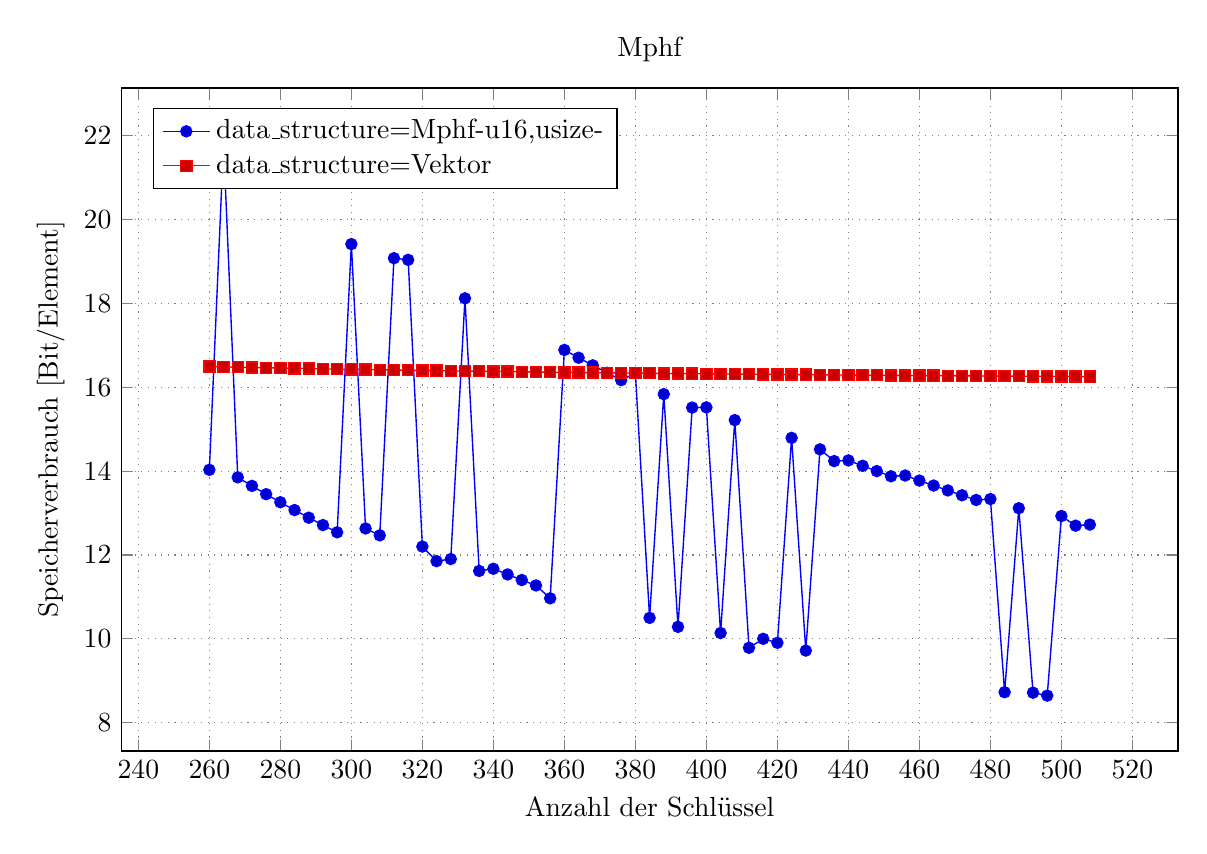
\begin{tikzpicture}
	\begin{axis}[
	title={Mphf},
	xlabel={Anzahl der Schlüssel},
	ylabel={Speicherverbrauch [Bit/Element]},
	]
	
	%% MULTIPLOT(data_structure) SELECT size AS x, size_bytes AS y, MULTIPLOT
	%% FROM mphf WHERE x % 4 == 0 AND x > 256 AND x < 512 GROUP BY MULTIPLOT,x ORDER BY MULTIPLOT,x
 \addplot coordinates { (260,14.0308) (264,21.8182) (268,13.8507) (272,13.6471) (276,13.4493) (280,13.2571) (284,13.0704) (288,12.8889) (292,12.7123) (296,12.5405) (300,19.4133) (304,12.6316) (308,12.4675) (312,19.0769) (316,19.038) (320,12.2) (324,11.8519) (328,11.9024) (332,18.1205) (336,11.619) (340,11.6706) (344,11.5349) (348,11.4023) (352,11.2727) (356,10.9663) (360,16.8889) (364,16.7033) (368,16.5217) (372,16.3441) (376,16.1702) (380,16.3368) (384,10.5) (388,15.8351) (392,10.2857) (396,15.5152) (400,15.52) (404,10.1386) (408,15.2157) (412,9.78641) (416,10.0) (420,9.90476) (424,14.7925) (428,9.71963) (432,14.5185) (436,14.2385) (440,14.2545) (444,14.1261) (448,14.0) (452,13.8761) (456,13.8947) (460,13.7739) (464,13.6552) (468,13.5385) (472,13.4237) (476,13.3109) (480,13.3333) (484,8.72727) (488,13.1148) (492,8.71545) (496,8.64516) (500,12.928) (504,12.6984) (508,12.7244) };
 \addlegendentry{data\_structure=Mphf-u16,usize-};
 \addplot coordinates { (260,16.4923) (264,16.4848) (268,16.4776) (272,16.4706) (276,16.4638) (280,16.4571) (284,16.4507) (288,16.4444) (292,16.4384) (296,16.4324) (300,16.4267) (304,16.4211) (308,16.4156) (312,16.4103) (316,16.4051) (320,16.4) (324,16.3951) (328,16.3902) (332,16.3855) (336,16.381) (340,16.3765) (344,16.3721) (348,16.3678) (352,16.3636) (356,16.3596) (360,16.3556) (364,16.3516) (368,16.3478) (372,16.3441) (376,16.3404) (380,16.3368) (384,16.3333) (388,16.3299) (392,16.3265) (396,16.3232) (400,16.32) (404,16.3168) (408,16.3137) (412,16.3107) (416,16.3077) (420,16.3048) (424,16.3019) (428,16.2991) (432,16.2963) (436,16.2936) (440,16.2909) (444,16.2883) (448,16.2857) (452,16.2832) (456,16.2807) (460,16.2783) (464,16.2759) (468,16.2735) (472,16.2712) (476,16.2689) (480,16.2667) (484,16.2645) (488,16.2623) (492,16.2602) (496,16.2581) (500,16.256) (504,16.254) (508,16.252) };
 \addlegendentry{data\_structure=Vektor};
 
	
	\end{axis}
	\end{tikzpicture}
\end{center}


\end{document}

%%%%%%%%%%%%%%%%%%%%%%%%%%%%%%%%%%%%%%%%%%%%%%%%%%%%%%%%%%%%%%%%%%%%%%%%%%%%%%%%
